\documentclass[class=report, crop=false, 12pt,a4paper]{standalone}
\usepackage{enumitem}
\usepackage{tikz}
\usepackage{float}
\usepackage{graphicx}
\usepackage{multicol}
\usepackage{siunitx}
\usepackage{mathtools}
\usepackage{amsmath}
\usepackage{amssymb}
\usepackage{commath}
\usepackage[normalem]{ulem}
\usepackage[a4paper,width=150mm,top=25mm,bottom=25mm]{geometry}
\begin{document}
\begin{center}
  23/11/2020
\end{center}
\section{Measurement of Velocity}
Linear- and angular-velocity transducers are available based on many different principles. Some of the more common types are introduced here. Linear velocity is often measured with an angular-velocity transducer by using a wheel to convert the linear motion into rotation. Angular-velocity transducers are given different names depending on their use:
\begin{itemize}
  \item Revolution counters – measure rates of rotation of a body by counting the rotation
  \item Tachogenerators – generate an output (typically voltage) proportional to the angular velocity of an element of the system
\end{itemize}
Mechanical rotation is coupled to an angular-velocity transducer via ‘sensing shaft’ which rotates at the angular velocity to be measured.
\subsection{Velocity transducers with a frequency output}
Similar principle to the angular position transducers, such as optical incremental shaft encoders, can be used to measure rotational frequency. 
\begin{figure}[H]
  \centering
  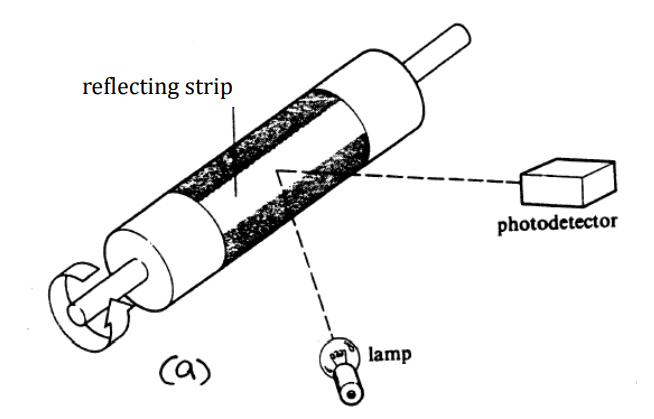
\includegraphics[width = 0.6\textwidth]{../img/Mdiagram43.png}
\end{figure}
Simple examples include a rotating shaft with a reflecting strip on non-reflecting background colour band (figure). Here, one electrical pulse per revolution is received by the detector.
\begin{figure}[H]
  \centering
  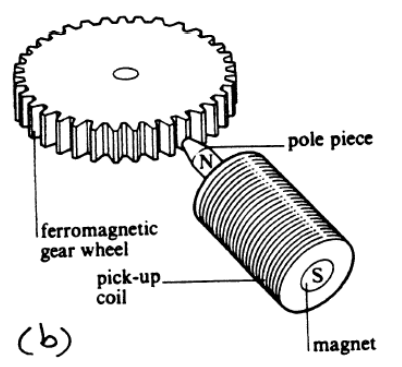
\includegraphics[width = 0.45\textwidth]{../img/Mdiagram44.png}
  \caption{A variable reluctance tachometer. A pick-up coil surrounds a permanent magnet, one pole of which is placed close to a ferromagnetic gear wheel mounted on the sensing shaft.}
\end{figure}
The reluctance of the magnetic circuit varies depending on the distance between the pole and gear tooth, and hence the magnetic flux inside the coil changes which induces the electromotive force (voltage).
\begin{figure}[H]
  \centering
  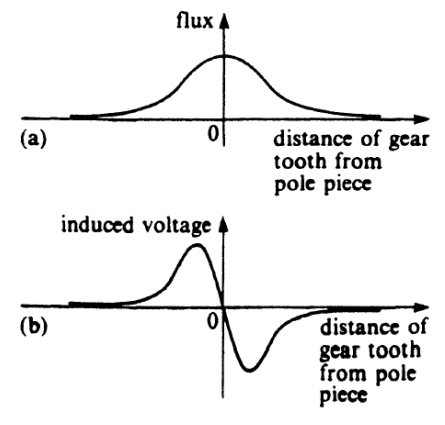
\includegraphics[width = 0.5\textwidth]{../img/Mdiagram45.png}
\end{figure}
The induced EMF (electromotive force) and voltage is proportional to the rate of change of flux, hence the distance between the gear and pole is related to the induced voltage via:
\begin{gather}
  \epsilon = -\frac{\dif}{\dif t}\text{(flux)}
\end{gather}
\subsection{Tachogenerator}
The tachogenerator generates a voltage (usually DC) proportional to angular velocity, using electromagnetic induction. The transducer uses the energy of rotation of the sensing shaft to generate an electrical output and requires no external power supply.
\begin{figure}[H]
  \centering
  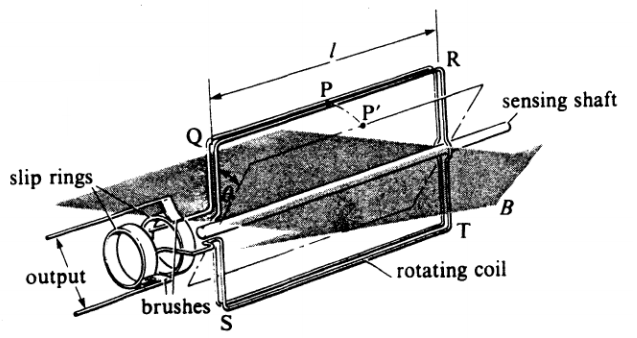
\includegraphics[width = 0.65\textwidth]{../img/Mdiagram46.png}
  \caption{Basic AC tachogenerator}
\end{figure}
Any conductor moving through a magnetic field at an angle $\theta$ to the direction of the field has an EMF induced as:
\begin{gather}
  \epsilon = Blv\sin(\theta)
\end{gather}
Where:
\begin{itemize}
  \item $B$ is the magnetic flux density
  \item $l$ is the length of the conductor 
  \item $v$ is the velocity of the conductor in the field
\end{itemize} 
If the conductor is moving parallel to the field, $\theta=0$ and no EMF is induced, whereas if it is moving normal to the field, $\theta = \pi/2$ and $\epsilon = Blv$. \\\\
In the tachogenerator, the induced voltage is picked up via two spring-loaded brushes, rubbing on two conducting rings called ‘slip rings’. The slip rings are connected to the two ends of the coil and rotate with it. The voltages generated in sides QR and ST are in the correct direction to add. The other two sides (QS and RT) do not contribute to the voltage.
\begin{figure}[H]
  \centering
  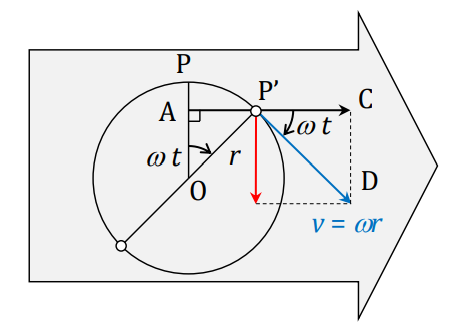
\includegraphics[width = 0.45\textwidth]{../img/Mdiagram47.png}
  \caption{Red arrow: $v\sin(\omega t)\longrightarrow$ Component crossing the magnetic field}
\end{figure}
From the figure, the induced EMF in the side QR can be calculated as: 
\begin{gather}
  \epsilon = Blv\sin(\theta) = Bl\omega r\sin(\omega t)
\end{gather}
With the contribution from the other side (ST), for $n$ turns of the coil:
\begin{gather}
  \text{Total induced voltage} = 2Bl\cdot n \cdot \omega r \cdot \sin(\omega t)
\end{gather}
From the equation, we can see that the output voltage is sinusoidal with amplitude proportional to the angular velocity $\omega$ (or frequency $f = \omega/2\pi$). \\\\
However, it is difficult to deal with an output where both the amplitude and frequency vary with angular velocity. It is more convenient to have DC output with its magnitude proportional to the angular velocity. \\\\
Modifications using \textbf{commutator} which switches over the two $(n)$ output terminals from the coil every half $(1/n)$ turn.
\begin{figure}[H]
  \centering
  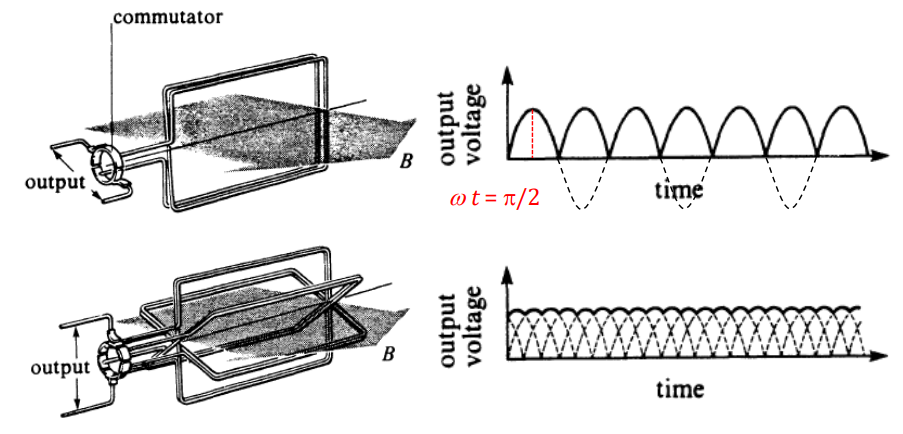
\includegraphics[width = 0.9\textwidth]{../img/Mdiagram48.png}
\end{figure}
\section{Measurement of Torque}
\subsection{Torque measurement with strain gauges}
Torque, a twisting force, can be measured by detecting the angular displacement or surface strain of a shaft that is subjected to a torque.
\begin{figure}[H]
  \centering
  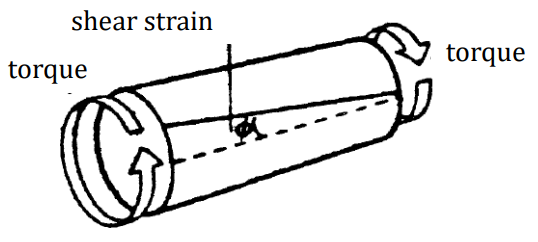
\includegraphics[width = 0.5\textwidth]{../img/Mdiagram49.png}
\end{figure}
For the use of strain gauge, it is necessary to know how much strain is present on the surface of the shaft for a given torque. \\\\
The relationship between torque $T$, shear strain (angle) $\phi$, shear modulus of the shaft material $G$ and radius $r$ is given as:
\begin{gather}
  T = \frac{1}{2}\pi Gr^3\phi 
\end{gather}
The shear sensitivity can be considered as the shear strain in the surface per unit applied torque:
\begin{gather}
  \text{Shear sensitivity} = \frac{\phi}{T} = \frac{2}{\pi Gr^3}
\end{gather}
A strain gauge will measure linear strain in the direction of the gauge axis. To maximise this for a given shear strain in the shaft, the gauge is mounted with its active axis $\ang{45}$ to the axis of the shaft.
\begin{figure}[H]
  \centering
  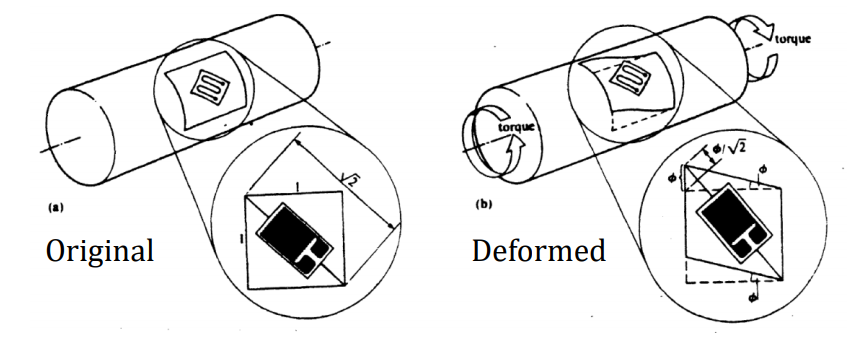
\includegraphics[width = 0.8\textwidth]{../img/Mdiagram50.png}
\end{figure}
Considering a unit square area on the surface and when $\phi$ is small, the strain in its diagonal is given as:
\begin{gather}
  e = \frac{\frac{\phi}{\sqrt{2}}}{\sqrt{2}} = \frac{\phi}{2}
\end{gather}
The gauge sensitivity can then be: 
\begin{gather}
  \frac{e}{T} = \frac{\phi}{2T} = \frac{1}{\pi Gr^3}
\end{gather}
Temperature compensation can be achieved by mounting two strain gauges with their active axes perpendicular to each other.
\begin{figure}[H]
  \centering
  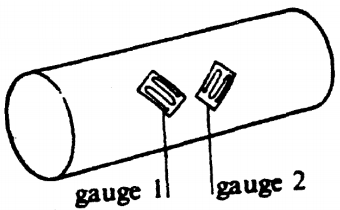
\includegraphics[width = 0.3\textwidth]{../img/Mdiagram51.png}
\end{figure}
\section{Measurement of Other Variables}
\subsection{Voltage – voltmeter}
Analogue voltmeter and ammeter are making use of electromagnetic force. Digital ones could be made with comparators.
\begin{itemize}
  \item Analogue Voltmeter - A coil is wrapped around an electromagnet, which is placed inbetween 2 poles of a magnet. The current passing through the coil generates an EMF, which moves the dial across, giving a reading of the voltage. 
  \item Digital Voltmeter - A comparator is used. The input voltage is passed through a series of comparators and through yes-no logic gates, the correct voltage is measured and displayed on a digital reader.
\end{itemize}
\begin{figure}[H]
  \centering
  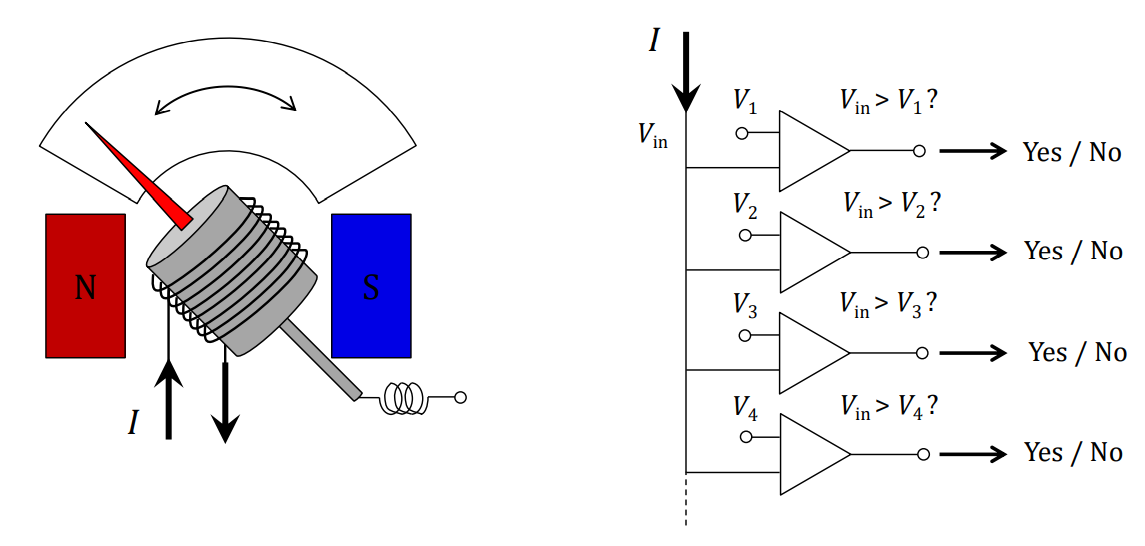
\includegraphics[width = 0.9\textwidth]{../img/Mdiagram52.png}
  \caption{Left-Analogue Voltmeter, Right-Digital Voltmeter}
\end{figure}
Advantages of digital voltage meters (DVMs) over analogue:
\begin{itemize}
  \item Read out of DVMs is easy as it eliminates observational errors in measurement committed by operators.
  \item Error on account of parallax and approximation is entirely eliminated.
  \item Reading can be taken very fast.
  \item Output can be fed to memory devices for storage and future computations.
  \item Versatile and accurate
  \item Compact and cheap
  \item Low power requirements
  \item Portability increased
\end{itemize}
\subsection{Light – photodiode}
LEDs or light emitting diodes make use of semiconductor blocks. Semiconductor blocks usually have a p-type and an n-type block. The n-type usually has an excess of electrons, whereas the p-type has extra capacity to hold electrons. When a current is passed through a circuit with semiconductor LED, the electrons move from the n-type to the p-type block, hence completing the circuit. 
\begin{figure}[H]
  \centering
  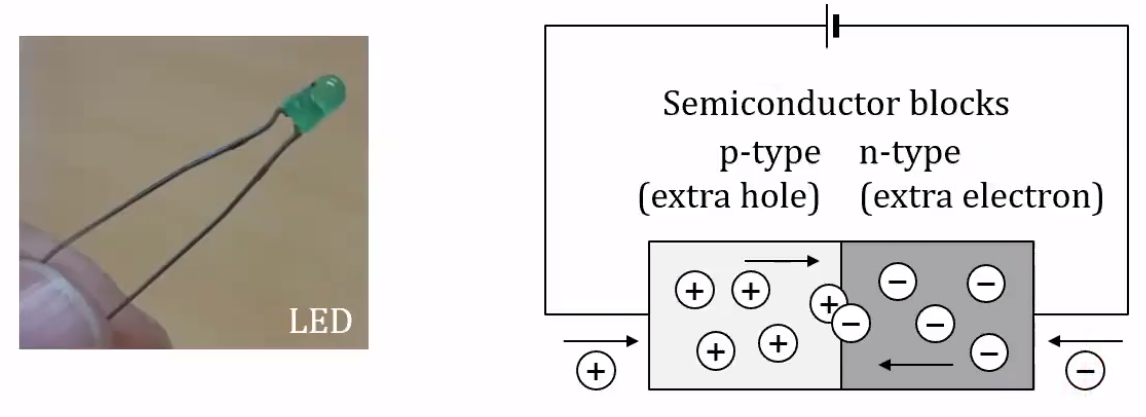
\includegraphics[width = 0.8 \textwidth]{../img/Mdiagram53.png}
\end{figure}
LED: Energy $\rightarrow$ Light
\begin{itemize}
  \item Type of semiconductors determines the amount of energy
  \item The amount of energy determines wavelength of the light $(E = hv)$
\end{itemize}
\subsubsection{What is the difference between and LED and a Photodiode/Phototransistor?}
A photodiode or a phototransistor work on opposite principles to an LED. When light is shone on the diode, it gets converted into energy and completes the circuit. So in this case, the light energy is used to push the electrons from the n-type semiconductor block to the p-type semiconductor block.
\begin{figure}[H]
  \centering
  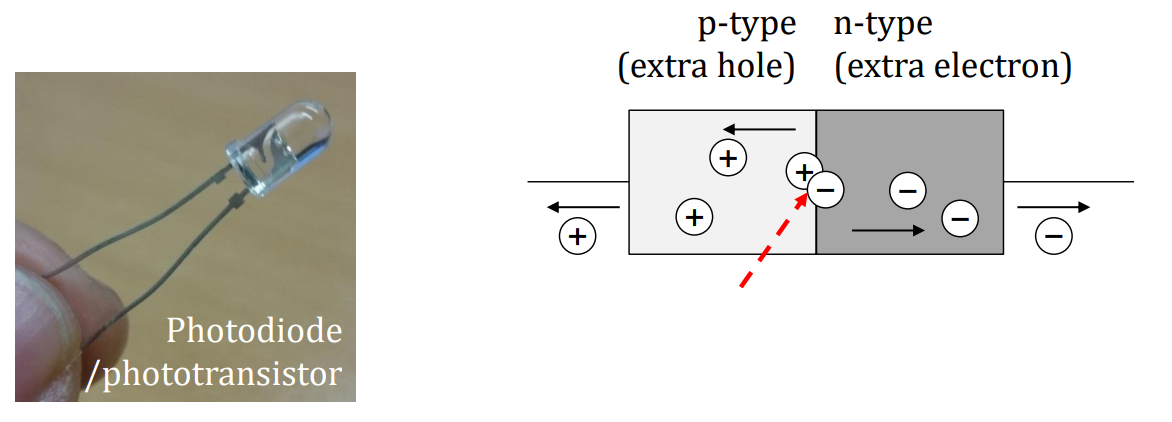
\includegraphics[width = 1 \textwidth]{../img/Mdiagram54.png}
\end{figure}
Photodiode: Light $\rightarrow$ Energy (photoelectric effect)
\begin{itemize}
  \item Pattern 1: Working as a power source $\longrightarrow$ photovoltaic mode – same principle in solar cells
  \item Pattern 2: Working as a switch $\longrightarrow$ photoconductive mode
\end{itemize}
\begin{figure}[H]
  \centering
  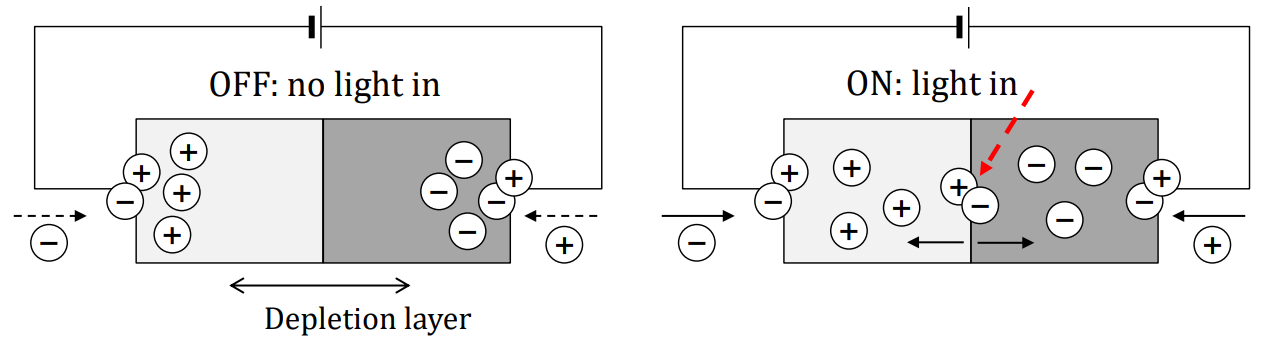
\includegraphics[width = 0.9 \textwidth]{../img/Mdiagram55.png}
\end{figure}
\subsection{Light – LDR (light dependent resistor)}
A light dependant resistor or an LDR changes its resistance depending on the intensity of light being shone on the semiconductor.
\begin{figure}[H]
  \centering
  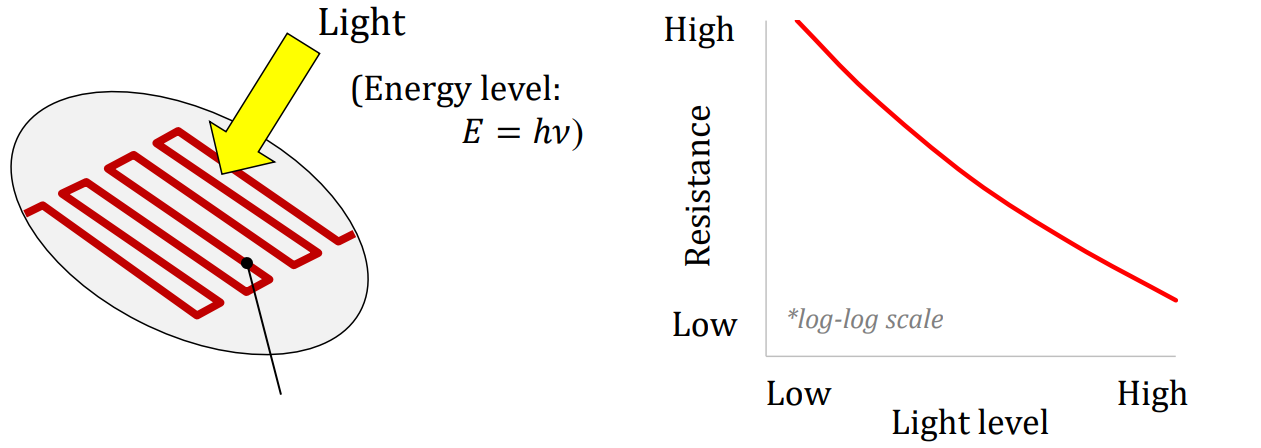
\includegraphics[width = 1 \textwidth]{../img/Mdiagram56.png}
\end{figure}
Semiconductor (CdS: cadmium sulfide) track:
\begin{itemize}
  \item Light energy excites electrons from the valence band to the conductive band
  \begin{itemize}
    \item Low resistance for high light level
  \end{itemize}
  \item Required energy level to “free up”
  electrons depends on the track material
  \begin{itemize}
    \item Semiconductor requires lower excitation energy than metal
  \end{itemize}
\end{itemize}
\subsection{Other Important Measurements}
\begin{itemize}
  \item Pressure Measurement
  \begin{itemize}
    \item Pitot tube
    \item Pressure probes (for healthcare applications)
  \end{itemize}
  \item Velocity/Flow Measurement
  \begin{itemize}
    \item Rotor
    \item Ultrasound doppler
    \item Optical approach
    \begin{itemize}
      \item Dye visualization
      \item Particle image velocimetry
    \end{itemize}
  \end{itemize}
\end{itemize}
\end{document}